\documentclass[10pt, letterpaper]{article}
\usepackage[utf8]{inputenc}
\usepackage[spanish,es-nodecimaldot]{babel}
\usepackage[top=1in, bottom=1in, left=1in, right=1in]{geometry}

\usepackage{csquotes}

\usepackage{amsmath}
\usepackage{amsthm}
\usepackage{amssymb}
\usepackage{graphicx}

\theoremstyle{definition}
\newtheorem{definition}{Definición}[section]


\begin{document}

\begin{center}
    {\large \bfseries Práctica 7: Particle Swarm Optimization (PSO) y Evolución Diferencial (DE) \par}
    \vspace{0.2cm}
    Facultad de Ciencias, UNAM - Pablo A. Trinidad - 10 Mayo 2019
\end{center}

\begin{enumerate}
    \item \textbf{[Ejercicio teórico]} Identifica y menciona cuáles son ls
    componentes de búsqueda relacionados con la exploración y la explotación
    del espacio de búsqueda en el algoritmo de PSO y DE respectivamente.
        \begin{itemize}
            \item \textbf{PSO}: La componente de explotación de este algoritmo
                  está dado por el hecho de que la velocidad de una partícula
                  es alterada tomando en cuenta su mejor posición hasta el momento
                  mientras que la exploración se da por el hecho de que se toma
                  en cuenta la posición de los vecinos, así como la posición de
                  la partícula con mejor \textit{fitness} dentro de todo
                  el \textit{swarm}.
            \item \textbf{DE}: La componente de explotación de éste algoritmo
                  está dada por el hecho de que una nueva solución particular
                  de un agente únicamente se aceptará si mejora el \textit{fitness},
                  mientras que la componente de exploración únicamente sucede
                  al inicio cuando los agentes son ubicados de manera aleatoria.
        \end{itemize}
    \item \textbf{[Ejercicio teórico]} ¿Cómo modificaría el algoritmo de PSO
    canónico visto en clase para incluir aceleración?\\
        \textbf{Respuesta:} Utilizaría la noción de tiempo y la definición
        de aceleración ($v=at$) para alterar cada $v_d$ de una partícula. Si
        $p_d$ disminuye (con la noción del espacio de búsqueda), entonces la
        aceleración también disminuiría.
    \item \textbf{[Ejercicio teórico]} ¿Cuál es la diferencia entre la versión
    síncrona y la versión asíncrona del algoritmo PSO?
        \textbf{Respuesta:} Como \cite{pso-sync-vs-async} menciona, un algoritmo
        de optimización síncrono es aquel que requiere un
        \textit{punto de sincronización} al final de cada iteración para reunir
        los resultados y actualizar las variables de control, por el contrario,
        el método asíncrono no requiere de un \textit{punto de sincronización}
        para determinar la nueva dirección de búsqueda o los nuevos valores de
        las valores de los parámetros de control por lo que los cómputos y las
        partículas pueden ser distribuidos a través de múltiples recursos.
        Adicionalmente y en el contexto particular de PSO la síncrona
        actualiza las velocidades y posiciones de las partículas al final de cada
        iteración, mientras que la asíncrona que actualiza la posición y velocidad
        de las partículas continuamente basado en la información disponible.
    \item \textbf{[Ejercicio de programación]} Implementar el algoritmo evolutivo
    diferencial básico y probar su funcionamiento minimizando las siguientes
    funciones (utiliza $d=30$):
        \begin{enumerate}
            \item Sphere:
                \begin{equation*} \begin{gathered}
                    f(\vec{x}) = \sum_{i=1}^{d} x_i^2
                \end{gathered} \end{equation*}
                donde $x_i \in [-100, 100]$
            \item Ackley:
                \begin{equation*} \begin{gathered}
                    f(\vec{x}) = -20 \cdot \exp \Bigg(
                        -0.2 \cdot
                        \sqrt{\frac{1}{d} \cdot \sum_{i=1}^{d} x_i^2}
                    \Bigg) -
                    \exp \Bigg(
                        \frac{1}{d} \cdot \sum_{i=1}^{d} \cos(2\pi x_i)
                    \Bigg) + 20 + \exp(1)
                \end{gathered} \end{equation*}
                donde $x_i \in [-30, 30]$
            \item Griewangk:
                \begin{equation*} \begin{gathered}
                    f(\vec{x}) = 1 + \frac{1}{4000} \sum_{i=1}^d x_1^2 -
                        \prod_{i=1}^d \cos \Bigg(\frac{x_i}{\sqrt{i}}\Bigg)
                \end{gathered} \end{equation*}
                donde $x_i \in [-600, 600]$
        \end{enumerate}
    Medir el mejor valor encontrado y el número de evaluaciones de función
    realizadas. Puedes utilizar los siguientes parámetros en tu algoritmo.
        \begin{itemize}
            \item Tamaño de población $=100$,
            \item $F=0.5$,
            \item Criterio de paro: máximo de iteraciones $500,000$ o tolerancia
            de error de $10^{-6}$ (lo que ocurra primero).
        \end{itemize}
    \textbf{Respuests:} Usando $F=0.75$ se obtuvieron los siguientes resultados:
    \begin{center} \begin{tabular}{ |c|c|c|c| }
        \hline
        Problema & Generaciones & Fitness promedio & Mejor fitness \\
        \hline
        Sphere  & 852 & 0.000066 & 0.00003 \\
        Ackley  & 885 & 0.0000719 & 0.0000478 \\
        Griewangk  & 938 & 0.0000464 & 0.0000272 \\
        \hline
    \end{tabular} \end{center}
    Adicionalmente se incluyen las animaciones de los resultados obtenidos
    en $d=1$ dentro del folder \texttt{GIFs}. Algo raro que sucedió en la función
    Ackley fue que el algoritmo convergía exageradamente rápido sin llegar al
    óptimo global, la mayoría de las veces ni siquiere pasaba de  2 iteraciones.
    Para evitar eso, se experimentó con los parámetros de control y se observó
    que con un \textbf{crossover probability}$=0.1$ finalmente
    el algoritmo comenzó a converger cerca del $0$ para todo $x_i$.
    \begin{center}
        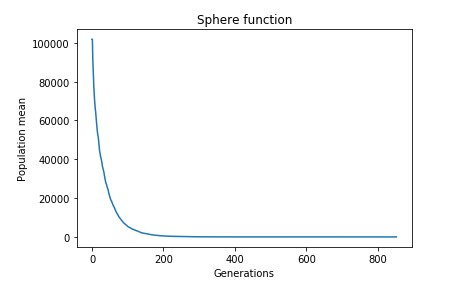
\includegraphics[scale=0.6]{assets/sphere-function.png}
    \end{center}
    \begin{center}
        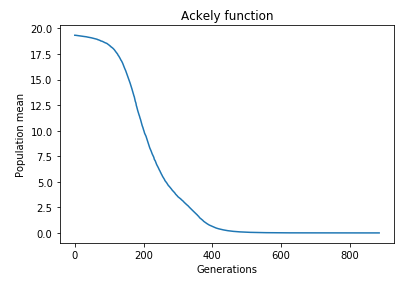
\includegraphics[scale=0.6]{assets/ackley-function.png}
    \end{center}
    \begin{center}
        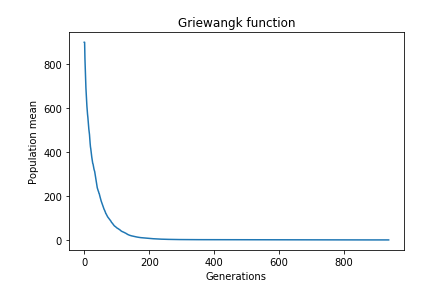
\includegraphics[scale=0.6]{assets/griewangk-function.png}
    \end{center}
    \item \textbf{[Ejercicio teórico]} Proponer una ligera moficación al
    algoritmo DE.\\
    \textbf{Respuesta:} Al igual que en las estrategias evolutivas, el parámetro
    de escala (\textit{differential weight}) puede ser parte del cromosoma
    de un individuo, dicho lo anterior reglas empíricas como la regla de los
    quintos podrían ser aplicadas.
    \item \textbf{[Ejercicio de programación]} Implementa el algoritmo propuesto
    y pruébalo con el mismo conjunto de funciones. Compara los resultados
    obtenidos entre \texttt{DE} canónico y tu propuesta (\texttt{CDE}).\\[\baselineskip]
    \textbf{Respuesta:} La comparasión de algoritmos trajo resultados
    muy particulares dependiendo del problema y la métrica a evaluar, a
    continuación se desglozan algunas de las observaciones y se recomienda
    visitar el \texttt{Jupyter Notebook} con los resultados completos obtenidos:
    \begin{enumerate}
        \item \textbf{Sphere}: Observamos que el número de generaciones
               o iteraciones que tuvo que ejecutarse cada algoritmo sufre una
               intersección al rededor de problemas de tamaño $d=15$. Para
               problemas de tamaño $d<15$ sucede que \texttt{CDE} tiende a
               ejecutarse un número mayor de iteraciones que \texttt{CE} aunque
               con un extraño \textit{patrón de picos} aparentemente cada
               múltiplo de 5. A partir de $d\geq 15$ los papeles cambian y la
               versión canónica suele requerir un número mayor de iteraciones al
               punto que para $d=30$ obtenemos que \texttt{CE} se ejecuta 840
               iteraciones mientras que \texttt{CDE} únicamente 587.
            \begin{center}
                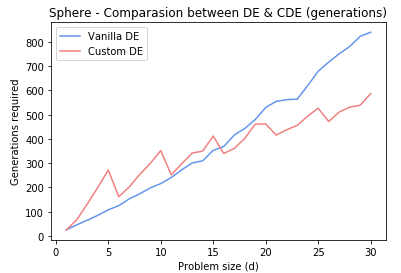
\includegraphics[scale=0.6]{assets/sphere-gens.png}
            \end{center}
            Y tal vez la pregunta natural que puede surgir es ¿cómo es que esto
            afecta a la calidad de las soluciones? Sabiendo que los óptimos
            de la función se encuentra en los valores $x_i=0$ para $i \in [1, d]$.
            Notamos que la calidad de la soluciones se intersectan al rededor del mismo
            punto de cruza mencionado anteriormente. A pesar de haberse ejecutarse por
            pocas iteraciones, \texttt{CDE} comienza encontrar mejores soluciones
            conforme el número de generaciones entre \texttt{DE} y \texttt{CDE}
            comienza a divergir. Es importante notar que antes de dicho punto
            de cruza, $d\approx 15$, \texttt{CDE} muestra dos intervalos con muy
            malas soluciones relativas a las encontradas por \texttt{DE}.
            \begin{center}
                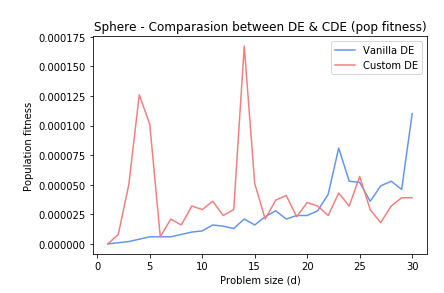
\includegraphics[scale=0.6]{assets/sphere-popfitness.png}
            \end{center}
            Por último podemos observar el mismo punto de cruza se mantiene
            respecto a la mejor solución encontrada al final de la ejecución,
            manteniendo también la dramática diferencia para $d=30$, siendo
            que \texttt{DE} obtuvo el mejor fitness con $0.000064$ mientras
            que \texttt{CDE} lo obtuvo con $0.0000013$.
            \begin{center}
                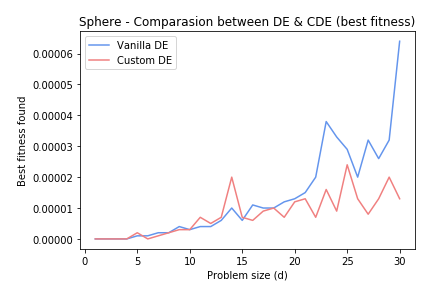
\includegraphics[scale=0.6]{assets/sphere-best.png}
            \end{center}
        \item \textbf{Ackley}: Respecto a las generaciones, \texttt{CDE} pareció
              mostrar siempre un número mayor de iteraciones requeridas antes
              de converger aunque con un extraño pico entre $d=25$ y $d=30$ donde
              parece que \texttt{CDE} convergió de manera extremadamente
              prematura afectando así el detalle las otras dos métricas, sin
              embargo, el experimento puede ser repetido para obtener más información
              respecto a este problema:
              \begin{center}
                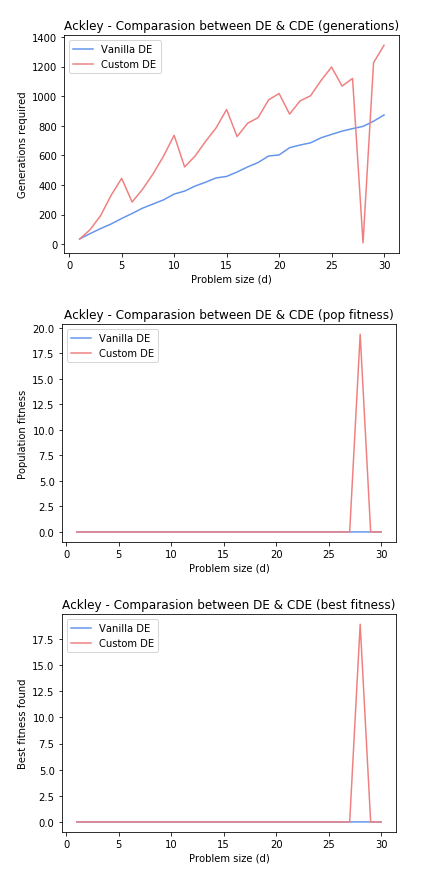
\includegraphics[scale=0.6]{assets/ackley-compound.png}
              \end{center}
        \item \textbf{Griewangk}: En este caso particular, los papeles se
              invirtieron respecto a Sphere en la primera métrica (número de iteraciones) ya que
              \texttt{CDE} converve después que \texttt{DE} para valores de
              $d\leq 17$ y luego sucede lo opuesto para valores $d>17$.
              \begin{center}
                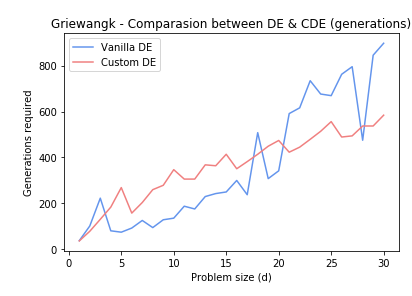
\includegraphics[scale=0.6]{assets/griewangk-gen.png}
              \end{center}
              Algo muy extraño sucedió respecto a la calidad de la soluciones
              y fue que \texttt{DE} convergió en muy malas soluciones la mayor
              parte del tiempo, mientras que \texttt{CDE} se mantuvo muy
              cerca del óptimo global sin importar la dimensión del problema.
              \begin{center}
                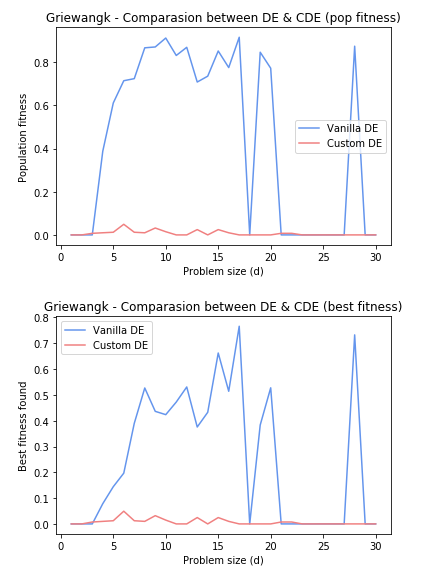
\includegraphics[scale=0.6]{assets/griewangk-fitness.png}
              \end{center}
              Dando diferencias tan extremas como la sucedida en $d=16$ donde
              \texttt{DE} obtuvo la mejor solución con valor $0.766072$ y
              \texttt{CDE} con valor $0.000009$, lo cuál también se reflejó
              en el fitness promedio con los mismos valores.
    \end{enumerate}
\end{enumerate}


% References
\clearpage
\begin{thebibliography}{9}
    \bibitem{hac-spso}
        Maurice Clerc.
        \textit{Standard Particle Swarm Optimisation.}
        2012. \texttt{hal-00764996}
    \bibitem{pso-sync-vs-async}
        Koh, B. I., George, A. D., Haftka, R. T., \& Fregly, B. J. (2006).
        \textit{Parallel asynchronous particle swarm optimization.}
        International journal for numerical methods in engineering,
        67(4), 578–595. doi:10.1002/nme.1646
\end{thebibliography}

\end{document}